\documentclass[fleqn]{article}
\usepackage[a4paper, left=1.5cm, right=1.5cm, top=1.5cm, bottom=1.5cm]{geometry}
\usepackage{amsmath}
\usepackage{helvet}
\usepackage{tikz}
\usepackage{bm}

\renewcommand{\familydefault}{\sfdefault}
\DeclareMathOperator*{\argmax}{arg\,max}
\usetikzlibrary{positioning}

\begin{document}

\section*{Setup BFE (current timestep $t=1$)}

\begin{figure}[htbp]
    \centering

    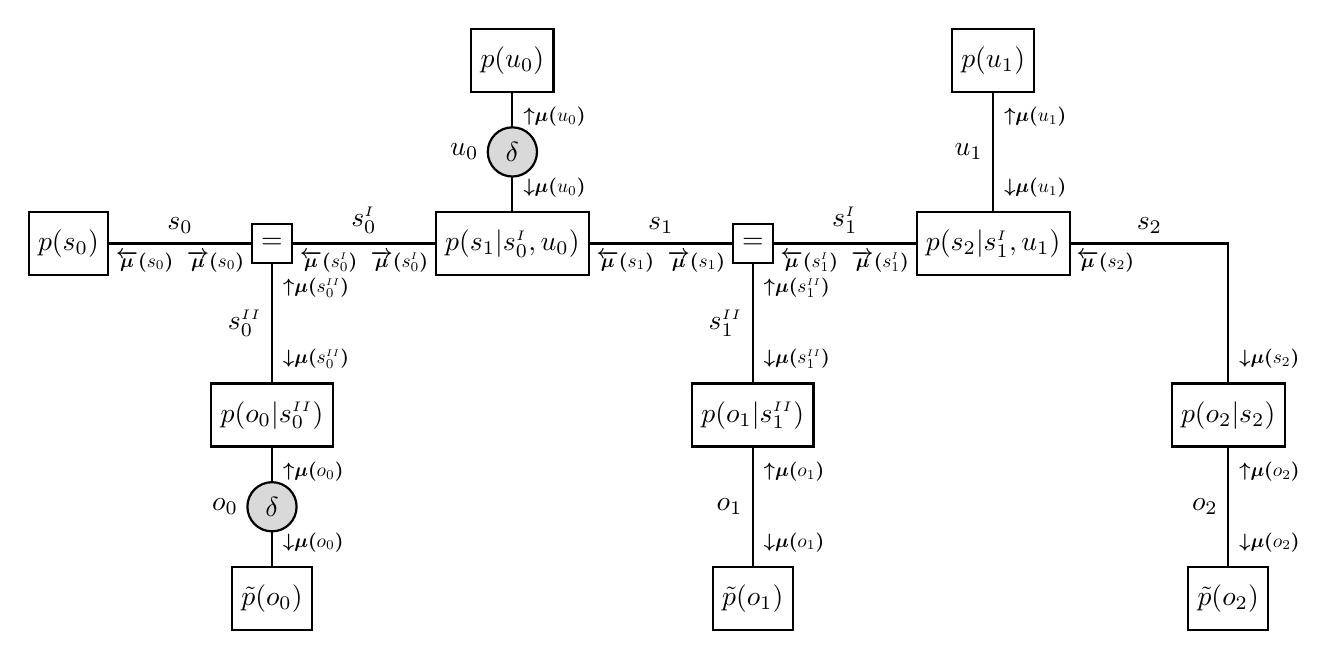
\begin{tikzpicture}[
            factor/.style={draw=black, thick, rectangle, minimum size=0.8cm, font=\normalsize},
            eqfactor/.style={draw=black, thick, rectangle, minimum size=0.5cm, font=\normalsize},
            edge/.style={thick},
            varlabel/.style={font=\normalsize},
            greycircle/.style={draw=black, thick, circle, fill=gray!30, minimum size=0.5cm, font=\normalsize}
        ]

        % Knoten
        \node[factor] (d) {$p(s_0)$};
        \node[eqfactor, right=1.8cm of d] (eq0) {$=$};
        \node[factor, below=1.5cm of eq0] (A0) {$p(o_0|s^{\scriptscriptstyle II}_0)$};
        \node[factor, below=1.5cm of A0] (c0) {$\tilde{p}(o_0)$};
        \node[factor, right=1.8cm of eq0] (B0) {$p(s_1|s^{\scriptscriptstyle I}_0,u_0)$};
        \node[eqfactor, right=1.8cm of B0] (eq1) {$=$};
        \node[factor, below=1.5cm of eq1] (A1) {$p(o_1|s^{\scriptscriptstyle II}_1)$};
        \node[factor, below=1.5cm of A1] (c1) {$\tilde{p}(o_1)$};
        \node[factor, right=1.8cm of eq1] (B1) {$p(s_2|s^{\scriptscriptstyle I}_1,u_1)$};
        \node[factor] (A2) at ([xshift=2cm] B1.east |- A1) {$p(o_2|s_2)$};
        \node[factor, below=1.5cm of A2] (c2) {$\tilde{p}(o_2)$};
        \node[factor, above=1.5cm of B0] (u0) {$p(u_0)$};
        \node[factor, above=1.5cm of B1] (u1) {$p(u_1)$};

        % Kanten zwischen Knoten
        \draw[edge] (d.east) -- (eq0.west) node[midway, above, varlabel] {$s_0$} node[near start, below, varlabel, scale=0.7] {$\bm{\overleftarrow{\mu}(}s_0\bm{)}$} node[near end, below, varlabel, scale=0.7] {$\bm{\overrightarrow{\mu}(}s_0\bm{)}$};

        \draw[edge] (eq0.south) -- (A0.north) node[midway, left, varlabel] {$s^{\scriptscriptstyle II}_0$} node[pos=0.2, right=0.05, varlabel, scale=0.7] {$\bm{{\uparrow}{\mu}(}s^{\scriptscriptstyle II}_0\bm{)}$} node[pos=0.8, right=0.05, varlabel, scale=0.7] {$\bm{{\downarrow}{\mu}(}s^{\scriptscriptstyle II}_0\bm{)}$} {};

        \draw[edge] (A0.south) -- (c0.north) node[midway, greycircle] {$\delta$} node[midway, left=0.3cm, varlabel] {$o_0$} node[pos=0.2, right=0.05, varlabel, scale=0.7] {$\bm{{\uparrow}{\mu}(}o_0\bm{)}$} node[pos=0.8, right=0.05, varlabel, scale=0.7] {$\bm{{\downarrow}{\mu}(}o_0\bm{)}$} {};

        \draw[edge] (eq0.east) -- (B0.west) node[midway, above, varlabel] {$s^{\scriptscriptstyle I}_0$} node[near start, below, varlabel, scale=0.7] {$\bm{\overleftarrow{\mu}(}s^{\scriptscriptstyle I}_0\bm{)}$} node[near end, below, varlabel, scale=0.7] {$\bm{\overrightarrow{\mu}(}s^{\scriptscriptstyle I}_0\bm{)}$};

        \draw[edge] (B0.north) -- (u0.south) node[midway, greycircle] {$\delta$} node[midway, left=0.3, varlabel] {$u_0$} node[pos=0.8, right=0.05, varlabel, scale=0.7] {$\bm{{\uparrow}{\mu}(}u_0\bm{)}$} node[pos=0.2, right=0.05, varlabel, scale=0.7] {$\bm{{\downarrow}{\mu}(}u_0\bm{)}$};

        \draw[edge] (B0.east) -- (eq1.west) node[midway, above, varlabel] {$s_1$} node[near start, below, varlabel, scale=0.7] {$\bm{\overleftarrow{\mu}(}s_1\bm{)}$} node[near end, below, varlabel, scale=0.7] {$\bm{\overrightarrow{\mu}(}s_1\bm{)}$};

        \draw[edge] (eq1.south) -- (A1.north) node[midway, left, varlabel] {$s^{\scriptscriptstyle II}_1$} node[pos=0.2, right=0.05, varlabel, scale=0.7] {$\bm{{\uparrow}{\mu}(}s^{\scriptscriptstyle II}_1\bm{)}$} node[pos=0.8, right=0.05, varlabel, scale=0.7] {$\bm{{\downarrow}{\mu}(}s^{\scriptscriptstyle II}_1\bm{)}$} {};

        \draw[edge] (A1.south) -- (c1.north) node[midway, left, varlabel] {$o_1$} node[pos=0.2, right=0.05, varlabel, scale=0.7] {$\bm{{\uparrow}{\mu}(}o_1\bm{)}$} node[pos=0.8, right=0.05, varlabel, scale=0.7] {$\bm{{\downarrow}{\mu}(}o_1\bm{)}$} {};

        \draw[edge] (eq1.east) -- (B1.west) node[midway, above, varlabel] {$s^{\scriptscriptstyle I}_1$} node[near start, below, varlabel, scale=0.7] {$\bm{\overleftarrow{\mu}(}s^{\scriptscriptstyle I}_1\bm{)}$} node[near end, below, varlabel, scale=0.7] {$\bm{\overrightarrow{\mu}(}s^{\scriptscriptstyle I}_1\bm{)}$};

        \draw[edge] (B1.east) -| (A2.north) node[pos=0.25, above, varlabel] {$s_2$} node[pos=0.11, below, varlabel, scale=0.7] {$\bm{\overleftarrow{\mu}(}s_2\bm{)}$} node[pos=0.915, right=0.05, varlabel, scale=0.7] {$\bm{{\downarrow}{\mu}(}s_2\bm{)}$} {};

        \draw[edge] (A2.south) -- (c2.north) node[midway, left, varlabel] {$o_2$} node[pos=0.2, right=0.05, varlabel, scale=0.7] {$\bm{{\uparrow}{\mu}(}o_2\bm{)}$} node[pos=0.8, right=0.05, varlabel, scale=0.7] {$\bm{{\downarrow}{\mu}(}o_2\bm{)}$} {};

        \draw[edge] (B1.north) -- (u1.south) node[midway, left, varlabel] {$u_1$} node[pos=0.8, right=0.05, varlabel, scale=0.7] {$\bm{{\uparrow}{\mu}(}u_1\bm{)}$} node[pos=0.2, right=0.05, varlabel, scale=0.7] {$\bm{{\downarrow}{\mu}(}u_1\bm{)}$};

        % Kanten an Knoten

    \end{tikzpicture}

    %\caption{CFFG}
    \label{fig:3}
\end{figure}

\noindent
\setlength{\jot}{0.7em}
\begin{minipage}[t]{0.5\textwidth}
    \begin{alignat}{2}
         & \rlap{\text{\bfseries Bethe Forward Sweep:}} \nonumber                                                                                                                                                                                         \\
         & \bm{\overrightarrow{\mu}(}s_0\bm{)}                        &  & = p(s_0)                                                                                                                                                                       \\
         & \bm{{\uparrow}{\mu}(}o_0\bm{)}                             &  & = \delta_{o_0, \hat{o_0}}                                                                                                                                                      \\
         & \bm{{\uparrow}{\mu}(}s^{\scriptscriptstyle II}_0\bm{)}     &  & = \exp \biggl(\sum_{o_0} q(o_0)\log p(o_0|s^{\scriptscriptstyle II}_0)\biggr)                                                                                                  \\
         & \bm{\overrightarrow{\mu}(}s^{\scriptscriptstyle I}_0\bm{)} &  & = \bm{\overrightarrow{\mu}(}s_0\bm{)} \bm{{\uparrow}{\mu}(}s^{\scriptscriptstyle II}_0\bm{)}                                                                                   \\
         & \bm{{\downarrow}{\mu}(}u_0\bm{)}                           &  & = \delta_{u_0,\hat{u}_o}                                                                                                                                                       \\
         & \bm{\overrightarrow{\mu}(}s_1\bm{)}                        &  & = \sum_{s^{\scriptscriptstyle I}_0, u_0} \bm{\overrightarrow{\mu}(}s^{\scriptscriptstyle I}_0\bm{)} \bm{{\downarrow}{\mu}(}u_0\bm{)} p(s_1|{s^{\scriptscriptstyle I}_0},u_0)   \\
         & \bm{{\uparrow}{\mu}(}o_1\bm{)}                             &  & = \tilde{p}(o_1)                                                                                                                                                               \\
         & \bm{{\uparrow}{\mu}(}s^{\scriptscriptstyle II}_1\bm{)}     &  & = \exp \biggl(\sum_{o_1} q(o_1)\log p(o_1|s^{\scriptscriptstyle II}_1)\biggr)                                                                                                  \\
         & \bm{\overrightarrow{\mu}(}s^{\scriptscriptstyle I}_1\bm{)} &  & = \bm{\overrightarrow{\mu}(}s_1\bm{)} \bm{{\uparrow}{\mu}(}s^{\scriptscriptstyle II}_1\bm{)}                                                                                   \\
         & \bm{{\downarrow}{\mu}(}u_1\bm{)}                           &  & = p(u_1)                                                                                                                                                                       \\
         & \bm{{\downarrow}{\mu}(}s_2\bm{)}                           &  & = \sum_{s^{\scriptscriptstyle I}_1, u_1} \bm{\overrightarrow{\mu}(}s^{\scriptscriptstyle I}_1\bm{)} \bm{{\downarrow}{\mu}(}u_1\bm{)} p(s_2|{s^{\scriptscriptstyle I}_1},u_1)   \\
         & \bm{{\downarrow}{\mu}(}o_2\bm{)}                           &  & = \exp \biggl( \sum_{s_2} q(s_2) \log p(o_1|s_2) \biggr)                                                                                                                       \\
         & \rlap{\text{\bfseries Bethe Backward Sweep:}} \nonumber                                                                                                                                                                                        \\
         & \bm{{\uparrow}{\mu}(}o_2\bm{)}                             &  & = \tilde{p}(o_2)                                                                                                                                                               \\
         & \bm{\overleftarrow{\mu}(}s_2\bm{)}                         &  & = \exp \biggl(\sum_{o_2} q(o_2)\log p(o_2|s_2)\biggr)                                                                                                                          \\
         & \bm{{\uparrow}{\mu}(}u_1\bm{)}                             &  & = \sum_{s^{\scriptscriptstyle I}_1, s_2} \bm{\overrightarrow{\mu}(}s^{\scriptscriptstyle I}_1\bm{)} \bm{\overleftarrow{\mu}(}s_2\bm{)} p(s_2|{s^{\scriptscriptstyle I}_1},s_2) \\
         & \bm{\overleftarrow{\mu}(}s^{\scriptscriptstyle I}_1\bm{)}  &  & = \sum_{u_1, s_2} \bm{{\downarrow}{\mu}(}u_1\bm{)} \bm{\overleftarrow{\mu}(}s_2\bm{)} p(s_2|s^{\scriptscriptstyle I}_1,u_1)
    \end{alignat}
\end{minipage}%
\begin{minipage}[t]{0.5\textwidth}
    \begin{alignat}{2}
         & \bm{{\downarrow}{\mu}(}s^{\scriptscriptstyle II}_1\bm{)}  &  & = \bm{\overrightarrow{\mu}(}s_1\bm{)} \bm{\overleftarrow{\mu}(}s^{\scriptscriptstyle I}_1\bm{)}                                  \\
         & \bm{{\downarrow}{\mu}(}o_1\bm{)}                          &  & = \exp \biggl( \sum_{s^{\scriptscriptstyle II}_1} q(s^{\scriptscriptstyle II}_1) \log p(o_1|s^{\scriptscriptstyle II}_1) \biggr) \\
         & \bm{\overleftarrow{\mu}(}s_1\bm{)}                        &  & = \bm{{\uparrow}{\mu}(}s^{\scriptscriptstyle II}_1\bm{)} \bm{\overleftarrow{\mu}(}s^{\scriptscriptstyle I}_1\bm{)}               \\
         & \bm{{\uparrow}{\mu}(}u_0\bm{)}                            &  & = \delta_{u_0, \hat{u}_o}                                                                                                        \\
         & \bm{\overleftarrow{\mu}(}s^{\scriptscriptstyle I}_0\bm{)} &  & = \sum_{u_o, s_1} \bm{{\downarrow}{\mu}(}u_0\bm{)} \bm{\overleftarrow{\mu}(}s_1\bm{)} p(s_1|s^{\scriptscriptstyle I}_0,u_0)      \\
         & \bm{{\downarrow}{\mu}(}s^{\scriptscriptstyle II}_0\bm{)}  &  & = \bm{\overrightarrow{\mu}(}s_0\bm{)} \bm{\overleftarrow{\mu}(}s^{\scriptscriptstyle I}_0\bm{)}                                  \\
         & \bm{{\downarrow}{\mu}(}o_0\bm{)}                          &  & = \delta_{o_0, \hat{o_0}}                                                                                                        \\
         & \bm{\overleftarrow{\mu}(}s_0\bm{)}                        &  & = \bm{{\uparrow}{\mu}(}s^{\scriptscriptstyle II}_0\bm{)} \bm{\overleftarrow{\mu}(}s^{\scriptscriptstyle I}_0\bm{)}               \\[0.5em]
         & \rlap{\text{\bfseries Updating Beliefs:}} \nonumber                                                                                                                                             \\
         & q(s_0)                                                    &  & \propto \bm{\overleftarrow{\mu}(}s_0\bm{)} \bm{\overrightarrow{\mu}(}s_0\bm{)}                                                   \\
         & q(s^{\scriptscriptstyle I}_0)                             &  & \propto \bm{\overleftarrow{\mu}(}s^{\scriptscriptstyle I}_0\bm{)} \bm{\overrightarrow{\mu}(}s^{\scriptscriptstyle I}_0\bm{)}     \\
         & q(s^{\scriptscriptstyle II}_0)                            &  & \propto \bm{{\uparrow}{\mu}(}s^{\scriptscriptstyle II}_0\bm{)} \bm{{\downarrow}{\mu}(}s^{\scriptscriptstyle II}_0\bm{)}          \\
         & q(s_1)                                                    &  & \propto \bm{\overleftarrow{\mu}(}s_1\bm{)} \bm{\overrightarrow{\mu}(}s_1\bm{)}                                                   \\
         & q(s^{\scriptscriptstyle I}_1)                             &  & \propto \bm{\overleftarrow{\mu}(}s^{\scriptscriptstyle I}_1\bm{)} \bm{\overrightarrow{\mu}(}s^{\scriptscriptstyle I}_1\bm{)}     \\
         & q(s^{\scriptscriptstyle II}_1)                            &  & \propto \bm{{\uparrow}{\mu}(}s^{\scriptscriptstyle II}_1\bm{)} \bm{{\downarrow}{\mu}(}s^{\scriptscriptstyle II}_1\bm{)}          \\
         & q(s_2)                                                    &  & \propto \bm{\overleftarrow{\mu}(}s_2\bm{)} \bm{{\downarrow}{\mu}(}s_2\bm{)}                                                      \\
         & q(u_0)                                                    &  & \propto \delta_{u_0,\hat{u_0}}                                                                                                   \\
         & q(u_1)                                                    &  & \propto \bm{{\uparrow}{\mu}(}u_1\bm{)} \bm{{\downarrow}{\mu}(}u_1\bm{)}                                                          \\
         & q(o_0)                                                    &  & \propto \delta_{o_0,\hat{o_0}}                                                                                                   \\
         & q(o_1)                                                    &  & \propto \bm{{\uparrow}{\mu}(}o_1\bm{)} \bm{{\downarrow}{\mu}(}o_1\bm{)}                                                          \\
         & q(o_2)                                                    &  & \propto \bm{{\uparrow}{\mu}(}o_1\bm{)} \bm{{\downarrow}{\mu}(}o_2\bm{)}
    \end{alignat}
\end{minipage}

\end{document}
